\chapter{\texttt{AUX} vs. \texttt{VERB}: Attempt at Separation of Verbs and Auxiliary Verbs (Experiment 4)}
\label{chap:failures}

We earlier mentioned how the line of distinction between verbs (POS tag \texttt{VERB}) and auxiliary verbs (POS tag \texttt{AUX}) is not well-defined in Section \ref{ssec:AuxVERB}. We shall treat this problem in this section, with a glance through some of the observations on the problem in Section \ref{ssec:auxverbsObservations}, followed by the definition of the working dataset in Section \ref{ssec:auxverbDataset}. We elaborate on the proposed solution to the problem, and the results of the experiment in Section \ref{ssec:auxverbExperiment} and \ref{ssec:auxverbResults} respectively. We finally conclude this section with a discussion of the results in \ref{ssec:auxverbDiscussion}.

\section{Observations About Problem Statement}
\label{ssec:auxverbsObservations}

According to the definition in UD\footnote{\url{https://universaldependencies.org/kpv/pos/AUX\_.html}}, \verb|AUX| is used as a common POS tag for verbal auxiliaries, as well as non-verbal TAME markers. The class of copulas are also included in this list.

This definition of auxiliaries is a bit different from \cite{langtypology} which separates the two classes of auxiliaries and copulas in different categories. The work also points out the correlation between the position of an inflected auxiliary in relation to the verb, and other word properties of the language, as first pointed by \cite{greenberg1963some}. In his work, \citeauthor{greenberg1963some} notes that the position of an inflected auxiliary in relation to the verb is generally the same as the position of verb in relation to an object. It is important to note that this generalization only holds for the inflected auxiliaries, and thus languages where the auxiliaries are not inflected are automatically ruled out from the consideration. \citeauthor{langtypology} points out the well-known exception to this generalization in case of verb-second languages like those of \verb|de|.

While the generalization made by \citeauthor{greenberg1963some} is a very good marker for possible identification of inflected auxiliaries, the requirement of identification of auxiliaries in noninflected form still remains as a problem. This problem can however, be mitigated in part by the usage of the list of tokens identified as auxiliary in a given language, as was started in UDv2.4 \citep{UDv2.4} with the help of a validator (cf. Level 5 checks in \verb|validate.py|\footnote{\url{https://github.com/UniversalDependencies/tools}} file). It must also be pointed out that since \citeauthor{greenberg1963some} did not extend this generalization to SVO languages, the generalization only holds for languages with VSO and SOV dominant word-order. Combining that with verb-second languages, the generalization can not be used globally across all the languages.

When the copulas are included in the definition of \verb|AUX|, the already difficult problem of separating \verb|AUX| and \verb|VERB| becomes even harder. In many languages, auxiliaries are a subset of verbs, with respect to specific usages. In other words, the same token can act as a verb or an auxiliary, depending upon the usage. The list of copula in many languages is also a subset of verbs, called as copulative verbs. However, as \citeauthor{langtypology} notes, there are cases of languages where the copula are not verbal in nature. The function of a copula can be realized by other means as well. The most common of these, viz. juxtaposition (example language- Ilocano), and use of predicators (example language- \verb|bm|) are listed in the work, where they may be combined with existing copulative verbs in the grammar of the language.

In essence, while the class \verb|AUX| in UD includes the copulative verbs, predicators, and other non-verbal TAME markers, the class \verb|VERB| is composed of open class categories of verbs.

\section{Dataset Definition}
\label{ssec:auxverbDataset}

This experiment was initially tried on \verb|hi|-HDTB treebank from UDv2.3 \citep{UDv2.3}, but failed terribly. With the release of UDv2.4 \citep{UDv2.4}, this experiment was tried again, keeping the dataset treebank same, but changing the model architecture among other parameters.

There are a few reasons for the choice of the language for the experiment. In \verb|hi|, we can more often than not draw a clear line of distinction between auxiliary as defined by UD, and the verbs. While the auxiliaries undergo inflection, and also include predicators and other TAME markers, they are restricted to a few tokens which rarely, if at all, are used as independent verbs. The factors as listed above, combined with the author's native fluency in the language makes it an ideal candidate for this experiment.

\section{Experiment}
\label{ssec:auxverbExperiment}

We approach the problem at hand as a classification problem. In the experiment, we create a classifier that tags the data in either of the three categories as \verb|AUX|, \verb|VERB| or neither of the two. Since the training data needs to contain the information on what instances to mark in either category and also differentiate tokens not marked as either UPOS tag, we label the data using NER tag format. As the classifier predicts the output label for each token, it also outputs a confidence score associated with each predicted label. By analysing the confidence score of each prediction and comparing it with the already annotated data, we should be able to point out the anomalies.

If we consider the gold-standard (GS) as erroneous as in present case, we need some data in a higher quality of annotation. A platinum standard is considered as a super-refined gold standard from which even the GS can be evaluated and verified. However, given a lack of such platinum standard, we restrict to a manual evaluation of the output of the classifier, using k-fold cross validation technique to test and train the classifier on the same data. We first split the data into 10 folds, and then proceed to label the data using NER format.

Between the two tagsets available for NER labelling, we choose IOBES format for the classification of the data in the following manner: All the instances marked as \texttt{AUX} are labelled as ``S-aux", and all the instances marked as \texttt{VERB} are labelled as ``S-verb". The rest of the tokens are labelled with `O' tag. We do not consider contiguous tokens as a continuous chain, and thus not use either of `I', `B' or `E' tags at all. This is also done so as to have better control over each token that the model learns to tag, thereby increasing the granularity of the data.

For the task of POS Tagging, Flair embeddings \citep{flair} were the state-of-the-art (SOTA) at the time of performing this experiment. The embeddings were shown to be outperform several models available at the time, across multiple NLP tasks, and therefore were the natural choice for this experiment. However, there are several hyper-parameters that can be tuned with respect to the models. We decided to tune the hyper-parameters with their corresponding choices as listed in Table \ref{tab:auxverbHyper}. The best choice for the hyper-parameter are also listed in the same table. 

\begin{longtable}{|l|p{6cm}|l|}
    \hline 
    \multicolumn{1}{|l|}{\textbf{Hyper-Parameter}} &
    \multicolumn{1}{p{6cm}|}{\textbf{Choices}} &
    \multicolumn{1}{l|}{\textbf{Tuned Value}} \\
    \hline 
    \endhead
    \hline 
    \multicolumn{3}{|r|}{{Continued on next page}} \\ 
    \hline
    \endfoot
    \endlastfoot
    \hline
    \label{tab:auxverbHyper}
        \multirow{2}{*}{\textbf{Embeddings}} & \textbf{Stack1:} Forward and Backward Flair Embedding trained on \verb|hi|-newswire & \multirow{2}{*}{Stack2}\\
        & \textbf{Stack2:} Word Embedding for \verb|hi|, Forward and Backward Flair Embedding trained on \verb|hi|-newswire & \\
        \hline
        \textbf{Use CRF?} & True, False & True\\
        \hline
        \textbf{Use RNN?} & True, False & True\\
        \hline
        \textbf{RNN Layers} & 1, 2, 4 & 2\\
        \hline
        \textbf{Size of Hidden Layer} & 32, 64, 128, 256 & 256\\
        \hline
        \textbf{Dropout} & Uniform Distribution in [0.0, 0.5] & 0.25\\
        \hline
        \textbf{Learning Rate} & 0.05, 0.1, 0.15, 0.2, 0.25 & 0.1\\
        \hline
    \caption{Hyper-Parameters for Neural Network}
\end{longtable}

With the optimized parameters, we train the model on each fold of the data, and test the trained model on the fold's test data. As mentioned earlier, the predicted output labels are accompanied with an associated confidence score that demonstrates the model's confidence in the predicted label. We here identify 6 categories of error patterns, based on the predicted label and the original label for the data, as listed in Table \ref{tab:auxverbCategories}.

\begin{longtable}{|l|l|l|}
\hline 
\multicolumn{1}{|l|}{\textbf{Category}} &
\multicolumn{1}{l|}{\textbf{Original}} &
\multicolumn{1}{l|}{\textbf{Prediction}} \\
\hline 
\endhead
\hline 
\multicolumn{3}{|r|}{{Continued on next page}} \\ 
\hline
\endfoot
\endlastfoot
    \hline
    \label{tab:auxverbCategories}
    aux\_TP & S-aux & S-aux \\
    O\_TP & O & O \\
    verb\_TP & S-verb & S-verb \\
    \hline
    \hline
    \multirow{2}{*}{aux-O} & O & S-aux \\
    & S-aux & O \\
    \hline
    \multirow{2}{*}{aux-verb} & S-aux & S-verb \\
    & S-verb & S-aux \\
    \hline
    \multirow{2}{*}{verb-O} & O & S-verb \\
    & S-verb & O \\
    \hline
    \caption{Categories of Error Patterns}
\end{longtable}

The associated confidence scores for each prediction can be used to detect the anomaly from what is labelled as per the original annotation, and what the classifier thinks should be the annotation label. For the cases where the original annotation is same as the classifier's prediction, we focus on the subset of the predictions where the confidence score is lower than 0.67. The idea is that since there are 3 categories, a prediction with the associated confidence lower than \(\frac{2}{3}\) might be erroneous. For the instances where there is a mismatch between the predicted label and the originally annotated label, we focus on instances with the confidence in prediction higher than 0.995. The idea in this case is that if the model is really sure about the prediction, the original annotation might be erroneous, and is worth looking into. Figure \ref{fig:auxvsverbsDistribution} shows the distribution of confidence scores for instances where the predicted label matches the original label, with the associated confidence value lower than 0.80. 

\begin{figure}[H]
    \centering
    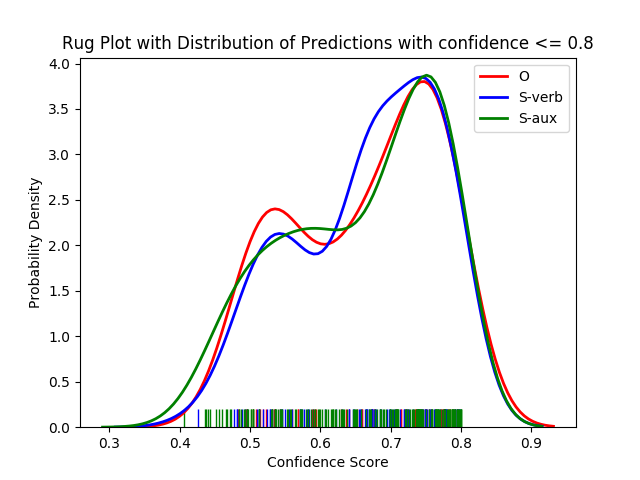
\includegraphics[scale=0.80]{img/aux-verb-distribution.png}
    \caption{Rug plot with Distribution of Predictions with low confidence score}
    \label{fig:auxvsverbsDistribution}
\end{figure}

Having identified instances within each category that have confidence scores within the relevant bound, these instances were manually annotated to see which one of the original annotation or the predicted annotation is correct. We can summarize the entire experiment in the form of algorithm as defined in Algorithm \ref{algo:auxverbAlgo}.

\begin{algorithm}[H]
\caption{Experiment to Identify Mislabelled \texttt{AUX} and \texttt{VERB} tags}
\label{algo:auxverbAlgo}
\begin{algorithmic}[1]
\REQUIRE $data \leftarrow$ UDv2.4 treebank
\STATE Convert $data.train$, $data.test$ and $data.dev$ to IOBES format
\STATE $model.config \leftarrow$ SOTA Classifier Configuration
\STATE $data.complete \leftarrow data.train + data.dev + data.test$
\STATE \COMMENT{The different splits of the data concatenated together}
\STATE $iter.id \leftarrow$ fold of $data.complete$, numbered as $id$
\STATE \COMMENT{Performed 10-fold cross-validation to split $data.complete$}
\STATE $model \leftarrow$ Classifier with configuration as per $model.config$
\FOR {$id$ in \{1, ... , 10\}}
    \STATE $model.id \leftarrow$ $model$ trained on $iter.id.train$ data
    \STATE $model.id.test \leftarrow$ Prediction of $model.id$ on $iter.id.test$ data
\ENDFOR
\STATE $identified.pure \leftarrow$ Original Annotation matches Prediction such that Confidence score \(\leq\) 0.6700
\STATE $identified.cross \leftarrow$ Original Annotation differs from Prediction such that Confidence score \(\geq\) 0.9950
\STATE Manual Annotation of $identified.pure$ and $identified.cross$
\end{algorithmic}
\end{algorithm}

\section{Results}
\label{ssec:auxverbResults}

The associated code for the experiment, alongwith the manually annotated data is available online\footnote{\url{https://github.com/Akshayanti/Masters-Thesis-CUNI-2020/tree/master/AUX-vs-VERB-UDv2.4}}. Given that the experiment is a case of a multi-class classification, the model performance is expressed in form of confusion metrics for each class \verb|AUX|, \verb|VERB| along with the metrics like Precision, Recall, Accuracy, F1 Score.

The metrics corresponding to the best performing model on the original treebank is listed in Table \ref{tab:auxverbBest}. When the models were trained on each of the folds, keeping the architecture of the best model, there was no loss in performance of the trained models (metric considered- micro averaged F1 score). 

% Change to a longtable if needed
\begin{table}[ht]
\centering
    \begin{tabular}{|l|c|c|c|c|}
        \hline
        \textbf{Label} & \textbf{Precision} & \textbf{Recall} & \textbf{Accuracy} & \textbf{F1 Score} \\
        \hline
        \verb|AUX| & 98.89 & 99.50 & 98.40 & 99.19 \\
        \verb|VERB| & 99.32 & 98.87 & 98.20 & 99.09 \\
        \hline
    \end{tabular}
\caption{Metrics of Best Model trained over original \texttt{hi} data}
\label{tab:auxverbBest}
\end{table}

As mentioned in previous section, we focused on the instances of the tagged data with confidence scores in particular bounds. Table \ref{tab:auxverbResults} lists the number of instances that were focused on in each category (as defined in Table \ref{tab:auxverbCategories}). The table also lists the number of instances that were identified as mislabelled, following the annotation procedure.

\newpage
\begin{longtable}{|c|c|c|c|}
\hline 
\multicolumn{1}{|l|}{\textbf{Category}} &
\multicolumn{1}{l|}{\textbf{Focused}} &
\multicolumn{1}{l|}{\textbf{Mislabelled}} &
\multicolumn{1}{l|}{\textbf{Percentage}} \\
\hline 
\endhead
\hline 
\multicolumn{4}{|r|}{{Continued on next page}} \\ 
\hline
\endfoot
\endlastfoot
    \hline
    \label{tab:auxverbResults}
    aux\_TP & 83 & 3 & 3.61 \\
    O\_TP & 25 & 5 & 20.00 \\
    verb\_TP & 45 & 10 & 22.22 \\
    \hline
    aux-O & 10 & 9 & 90.00 \\
    aux-verb & 42 & 23 & 54.76 \\
    verb-O & 20 & 11 & 55.00 \\
    \hline
    \hline
    \textbf{Overall} & 225 & 61 & 27.11 \\
    \hline
\caption{Results of Manual Annotation}
\end{longtable}

\section{Discussion of the Results}
\label{ssec:auxverbDiscussion}

\begin{table}[h]
    \centering
    \begin{tabular}{|l|l|}
        \hline
        \textbf{Metric} & \textbf{Count} \\
        \hline
        Sentences & 16 647 \\
        Words & 351 704 \\
        Tagged \verb|AUX| & 26 030 \\
        Tagged \verb|VERB| & 33 753 \\
        \hline
    \end{tabular}
    \caption{Statistics for \texttt{hi} data}
    \label{tab:auxverbDetails}
\end{table}

Table \ref{tab:auxverbDetails} lists the counts of sentences and the number of \verb|AUX| and \verb|VERB| tags in the entire \verb|hi|-HDTB treebank. Of the total number of tags listed in either category, we are able to focus on just 225 instances where we might be able to identify the problems. Even out of those 225 identified instances, just a bit over 25\% are actually erroneous. 

While hypertuning the best configuration of the classifier, the parameters correspond to the F1 score on how well it fits to the original data. Essentially, the best performing model is biased in the way that it would always try to find a prediction that matches the original annotation. While there is no other way on how to hypertune the model, the experimental results are therefore liable to find comparatively less instances where the confidence score is within the bounds as considered in the experiment. 

Further, the lack of a definable baseline for the attempted solution of the given problem makes it difficult for the current approach to be compared against a benchmark. Considering the lack of benchmark, we can crudely estimate the performance of the experiment by the ratio of the number of errors that were found in the focused cases to the number of instances that were focused on. 

While certain patterns are more reliable than others (the case where predicted output doesn't match the original annotation), the overall performance for the experiment is low as can be attributed to different factors mentioned above. Given the low scout-ability of the error cases in the experiment, the approach used in the experiment is not reliable enough for the process to be automated.